\section{Практика}

\begin{figure}
	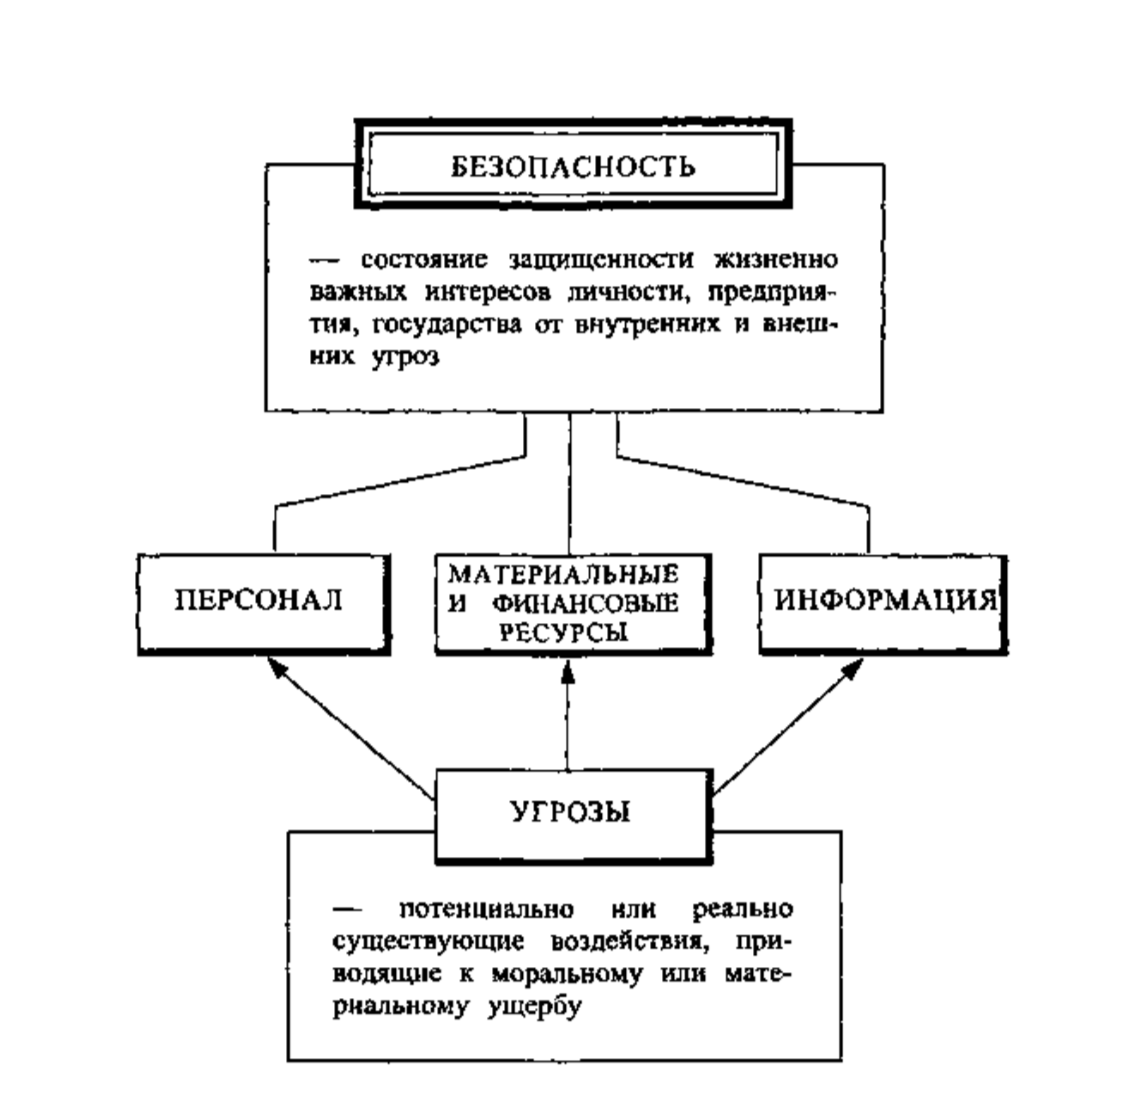
\includegraphics[width=\textwidth]{img/main_scheme.png}
	\caption{Угрозы безопасности}	
\end{figure}

\subsection{Аудит безопасности}

Для получения согласия клиента на проведения аудита было сформулировано сообщение следующего содержания:  <<Аудит позволяет оценить текущую безопасность функционирования информационной системы, оценить и прогнозировать риски, управлять их влиянием на бизнес-процессы фирмы, корректно и обоснованно подойти к вопросу обеспечения безопасности ее информационных активов, стратегических планов развития, маркетинговых программ, финансовых и бухгалтерских ведомостей, содержимого корпоративных баз данных. В конечном счете, грамотно проведенный аудит безопасности информационной системы позволяет добиться максимальной отдачи от средств, инвестируемых в создание и обслуживание системы безопасности фирмы.>>

После получение согласия клиента была формализована методика проверки, включающая в себя:

\begin{itemize}
	\item Сбор информации (Google, WWW, DNS);
	\item Сканирование системы (ping, port scanning);
	\item Получение доступа (эксплуатация уязвимости);
	\item Закрепление в системе (backdoor);
	\item Скрытие следов пребывания (очистка лог-файлов, rootkit).
\end{itemize}

\subsubsection{Пассивный и активный сборы информации}

Прежде чем начать активный взлом системы, нам надо собрать как можно больше информации о нашей цели. Можно сказать, что от того, насколько хорошо мы будем знать нашу цель, напрямую будет зависеть успех или провал всего мероприятия. Это самый важный этап аудита системы, на который чаще всего уходит большая часть времени.

Условно сбор информации делят на активную и пассивную фазы. Во время пассивной фазы наша «цель» не знает о том, что мы начали сбор информации. На данном этапе мы используем информацию только из отрытых и общедоступных источников, таких как поисковые системы и базы данных NIC. Также к пассивному сбору информации можно отнести сниффинг — когда мы просто перехватываем всю приходящую на наш сетевой интерфейс информацию и при этом ничего сами в сеть не посылаем.

Под активным сбором информации подразумевается непосредственное взаимодействие с системой. И скорее всего, данная активность будет занесена в журнал целевой системы.

К данной фазе можно отнести сканирование портов, определение работающих сервисов и их версий, а также определение версии операционной системы, под управлением которой работают данные сервисы.

\subsubsection{Сканирование системы}

Предположим, что, используя добытую на первом этапе информацию, мы получили из открытой базы данных RIPE диапазон IP-адресов целевой организации. После этого мы начинаем сканирование всей подсети предприятия.

На данном этапе чаще всего используются:
\begin{itemize}
	\item сканеры открытых портов;
	\item ICMP-сканеры;
	\item SNMP-сканеры;
	\item сканеры уязвимостей и т. д.
\end{itemize}

Во время данного этапа аудитор может получить следующую информацию:
\begin{itemize}
	\item имена компьютеров;
	\item версию операционной системы;
	\item запущенные сервисы и их версии;
	\item IP-адреса;
	\item учетные записи пользователей и т. д
\end{itemize}

\subsubsection{Получение доступа}

После получения информации в результате предыдущего этапа мы можем использовать ее для проникновения в систему. Например, мы узнали, что на одном из хостов установлен IIS. Используя версию и название сервиса, можно найти уязвимость, а затем и поэксплуатировать ее.

Одни из самых популярных методов — перехват сессии, переполнение буфера и отказ от обслуживания.

\subsubsection{Закрепление в системе}

Поскольку редко получается проникнуть в систему с наскока, мы хотим использовать повторно полученный однажды доступ. Нам нужна возможность продолжить начатое ранее тестирование, не прибегая к очередному взлому той же самой системы.

\subsubsection{Скрытие следов пребывания}

Итак, мы получили доступ к обозначенной системе и контролируем ее. Разумеется, мы не хотим, чтобы кто-то из ИТ-персонала компании заметил наше присутствие.
В противном случае мы можем потерять доступ не только к полученной системе, но и к сети в принципе.
Чаще всего стирают следы присутствия из журналов системы, а также события из базы данных IDS (системы обнаружения атак).

\subsection{Проверка векторов атаки}

\subsubsection{Доверенная загрузка}

SecureBoot\footnote{https://ru.wikipedia.org/wiki/Secure\_boot} — это программная технология, при помощи которой UEFI-совместимая прошивка может проверить подлинность исполняемых ей внешних компонентов (загрузчиков, драйверов и UEFI OptionROM'ов). Эти исполняемые компоненты должны быть подписаны ЭЦП, которая проверяется во время загрузки и в случае ее полного отсутствия, повреждения, отсутствия в списке доверенных (db) или присутствия в списке запрещенных (dbx) запуск соответствующего компонента не происходит. 

В проверяемых мной системах доверенная загрузка была включена.

\subsubsection{Сервис SSH}

OpenSSH\footnote{https://ru.wikipedia.org/wiki/OpenSSH} - свободно распространяемая версия семейства инструментов для удаленного управления компьютерами и передачи файлов с использованием протокола безопасной оболочки (SSH). Традиционные инструменты, используемые для этих функций, такие как telnet\footnote{https://ru.wikipedia.org/wiki/Telnet} и rcp\footnote{https://en.wikipedia.org/wiki/Berkeley\_r-commands}, незащищены и передают пользовательский пароль открытым текстом. OpenSSH предоставляет сервис на сервере и клиентские приложения для облегчения операций защиты, зашифрованного удаленного управления и передачи файлов, эффективно заменяя устаревшие инструменты.

\subsubsection{SELinux}

SELinux\footnote{https://ru.wikipedia.org/wiki/SELinux} — это система принудительного контроля доступа, реализованная на уровне ядра. Впервые эта система появилась в четвертой версии CentOS, а в 5 и 6 версии реализация была существенно дополнена и улучшена. Эти улучшения позволили SELinux стать универсальной системой, способной эффективно решать массу актуальных задач. Стоит помнить, что классическая система прав Unix применяется первой, и управление перейдет к SELinux только в том случае, если эта первичная проверка будет успешно пройдена.



\subsection{Устранение брешей}

\subsubsection{Сервис SSH}

В первую очередь следуют защититься от систематически повторяющихся попыток подбора пароля - bruteforce\footnote{https://en.wikipedia.org/wiki/Brute-force\_attack}.

Сервис Fail2ban может смягчить эту угрозу при помощи правил, автоматически меняющих настройки брандмауэра iptables\footnote{https://ru.wikipedia.org/wiki/Iptables}; эти правила срабатывают в случае поступления определённого количества неудачных попыток входа. Этот инструмент позволяет защитить сервер от несанкционированного доступа без вмешательства системного администратора.

Инструмент Fail2ban не доступен в официальном репозитории CentOS, но его можно получить в EPEL. Пакет самого репозитория EPEL (Extra Packages for Enterprise Linux) можно добавить из официального репозитория CentOS.

\begin{lstlisting}
sudo yum install epel-release
\end{lstlisting}

Теперь можно установить пакет fail2ban:

\begin{lstlisting}
sudo yum install fail2ban
\end{lstlisting}

После завершения установки следует использовать инструмент systemctl, чтобы включить fail2ban.

\begin{lstlisting}
sudo systemctl enable fail2ban
\end{lstlisting}

Сервис fail2ban хранит настройки в каталоге /etc/fail2ban. В нём можно найти файл jail.conf, содержащий стандартные настройки.

Этот файл перезаписывается при обновлении пакета Fail2ban, потому его редактировать нельзя. Вместо этого нужно создать новый файл по имени jail.local. Значения в файле jail.local будут переопределять jail.conf.

Файл jail.conf содержит раздел [DEFAULT], после которого следует раздел для индивидуальных сервисов. Файл jail.local может переопределить любое из этих значений. Файлы применяются в алфавитном порядке:

\begin{enumerate}
	\item /etc/fail2ban/jail.conf
	\item 	/etc/fail2ban/jail.d/*.conf,
	\item 	/etc/fail2ban/jail.local
	\item 	/etc/fail2ban/jail.d/*.local,
\end{enumerate}

Теперь изменим настройки sshd. 
Будет редактировать файл $ssh_config$.
\begin{lstlisting}
nano /etc/ssh/sshd_config.
\end{lstlisting}

Поменяем порт для подключения по умолчанию.

\begin{lstlisting}
Port 1337
\end{lstlisting}

Превентивно заставим использовать протокол второй версии.

\begin{lstlisting}
Protocol 2
\end{lstlisting}

Отменим удалённое подключение для root пользователя.

\begin{lstlisting}
PermitRootLogin no
\end{lstlisting}

\subsubsection{SELinux}

SELinux имеет три основных режим работы, при этом по умолчанию установлен режим
\textbf{Enforcing}. Это довольно жесткий режим, и в случае необходимости он может быть изменен на более удобный для конечного пользователя.

\textbf{Enforcing}: Режим по умолчанию. При выборе этого режима все действия, которые каким-то образом нарушают текущую политику безопасности, будут блокироваться, а попытка нарушения будет зафиксирована в журнале.

\textbf{Permissive}: В случае использования этого режима, информация о всех действиях, которые нарушают текущую политику безопасности, будут зафиксированы в журнале, но сами действия не будут заблокированы.

\textbf{Disabled}: Полное отключение системы принудительного контроля доступа.

Текущий статус можно посмотреть командой \textbf{sestatus}.

\begin{lstlisting}
SELinux status:                 enabled
SELinuxfs mount:                /selinux
Current mode:                   enforcing
Mode from config file:          enforcing
Policy version:                 21
Policy from config file:        targeted
\end{lstlisting}

SELinux далеко не так страшен, как о нем говорят. Система хоть и сложна в понимании, но невероятно логична и удобна в сопровождении, а имеющиеся средства управления позволяют очень точно диагностировать проблемы и легко их устранять.
